\documentclass[Report.tex]{subfiles}

\newcommand{\newaxis}[4]{
\begin{axis}[
    ybar,
    title={#1},
    ymin=#3, ymax=#4,
    bar width=1em,
    legend style={at={(0.5,-0.25)},anchor=north,legend columns=-1},
    enlarge x limits=0.4,
    x tick label style={align=center,text width=1.7cm},
    symbolic x coords={Logistic Regression, Random Forest, Multi-layer Perceptron},
    xtick=data,
    ylabel={#2}
]
}
% Read data
%\newcommand{\accprerecbarplot} {
%  \addplot+[
%    discard if not={feature}{#1},
%] table [x expr=\coordindex, y={accuracy}] {};
%}

\pgfplotstableread[col sep=comma]{data/15-pair-cv.csv}\fifteenPairCV

\begin{document}

\section{Player identification}
This section describes the different experiments conducted and analyses their results. For all experiments, the dataset is split into training and testing data. When splitting the dataset for pair classification (TODO reference section), no players in the training set appear in the testing set. All experiments used a two-step evaluation method to obtain metrics for training and testing.
\begin{enumerate}
\item During training, evaluation metrics were gathered using a 5-fold cross evaluation. This gives an idea on how well the models and feature perform, but the performance is likely inflated as the same player may appear in both the training and evaluation data. A 5-fold cross evaluation was chosen to give a balance between the amount of data used for training and evaluation (80\% and 20\% respectively for each fold) and performing enough runs to get a strong average. 
\item After the 5-fold cross evaluation, the final model is trained using all the training data, and evaluated against the testing data. This is the best indication of how the models perform against unseen data, as the testing data is untouched until this point of the experiment. 
\end{enumerate}

\subsection{Mouse movement features}\label{sec:mm-features-results}
The first experiments and results looked only at using the mouse movement features to see how effective they were at predicting the player. As there are three types of level 3 mouse movement feature (MMAC, MMMC and MMSC) as described in section \ref{sec:mm-features}, each feature is first evaluated individually and together, to see which feature may be more important to player prediction. 

\subsubsection{Individual movements}
 
\begin{figure}[H]
\begin{subfigure}{1\textwidth}
\centering
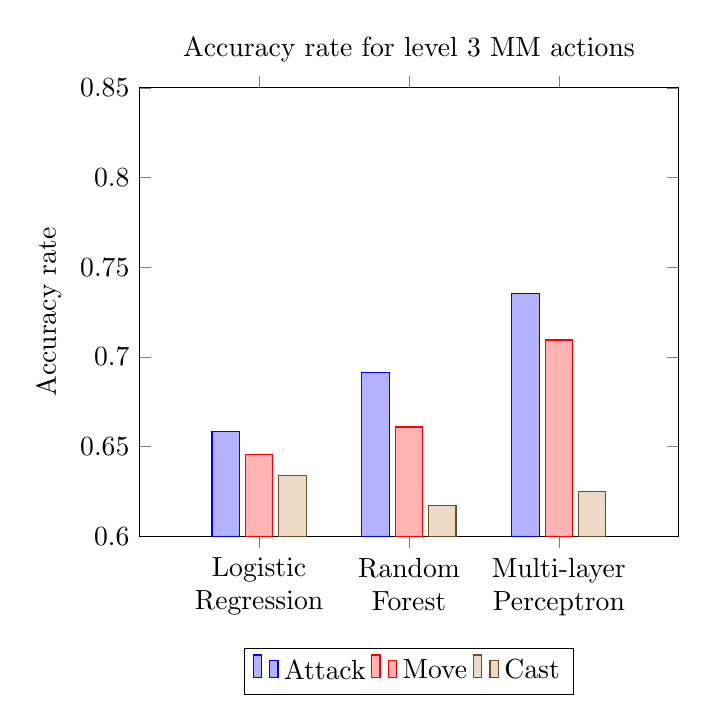
\begin{tikzpicture}
\newaxis{Accuracy rate for level 3 MM actions}{Accuracy rate}{0.6}{0.85}

\addplot coordinates {(Logistic Regression,0.6586) (Random Forest,0.6915) (Multi-layer Perceptron,0.7355)};
\addplot coordinates {(Logistic Regression,0.6457) (Random Forest,0.6609) (Multi-layer Perceptron,0.7094)};
\addplot coordinates {(Logistic Regression,0.6339) (Random Forest,0.6173) (Multi-layer Perceptron,0.6248)};
\legend{Attack,Move,Cast}

\end{axis}
\end{tikzpicture}
\end{subfigure}
\hspace{\fill}
\begin{subfigure}{0.45\textwidth}
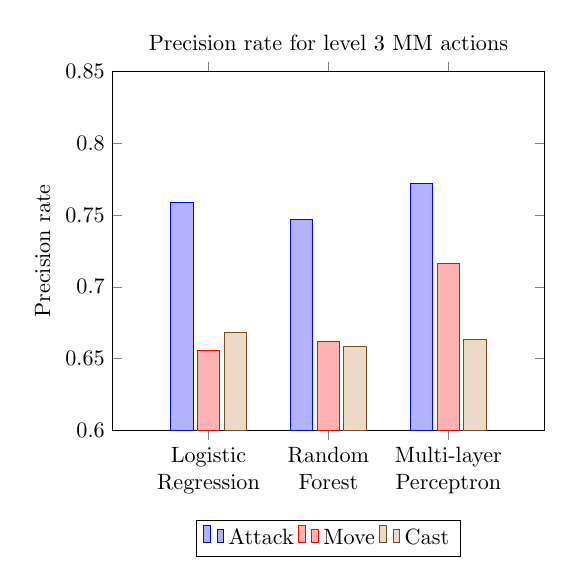
\begin{tikzpicture}[scale=0.8]
\newaxis{Precision rate for level 3 MM actions}{Precision rate}{0.6}{0.85}

\addplot coordinates {(Logistic Regression,0.759) (Random Forest,0.747) (Multi-layer Perceptron,0.7719)};
\addplot coordinates {(Logistic Regression,0.65524) (Random Forest,0.6618) (Multi-layer Perceptron,0.7165)};
\addplot coordinates {(Logistic Regression,0.6683) (Random Forest,0.6582) (Multi-layer Perceptron,0.6633)};
\legend{Attack,Move,Cast}

\end{axis}
\end{tikzpicture}
\end{subfigure}
\hspace{\fill}
\begin{subfigure}{0.45\textwidth}
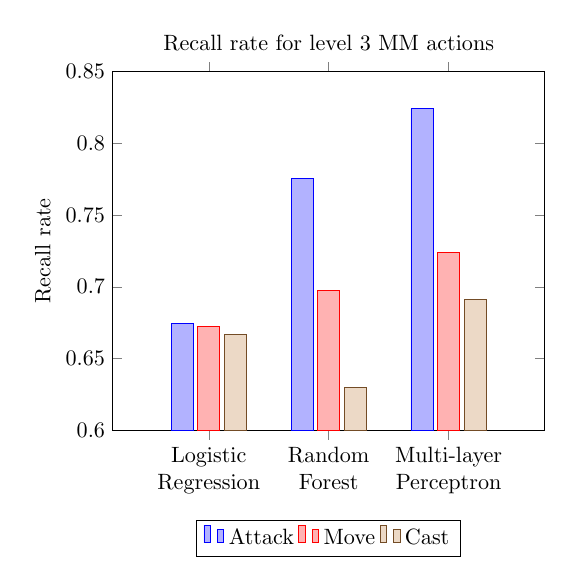
\begin{tikzpicture}[scale=0.8]
\newaxis{Recall rate for level 3 MM actions}{Recall rate}{0.6}{0.85}
\addplot coordinates {(Logistic Regression,0.6747) (Random Forest,0.7754) (Multi-layer Perceptron,0.8243)};
\addplot coordinates {(Logistic Regression,0.672) (Random Forest,0.6975) (Multi-layer Perceptron,0.7239)};
\addplot coordinates {(Logistic Regression,0.6665) (Random Forest,0.6301) (Multi-layer Perceptron,0.6909)};
\legend{Attack,Move,Cast}
\end{axis}
\end{tikzpicture}
\end{subfigure}
\caption{Classification rates using only mouse movement features.}
\label{fig:move-results}
\end{figure}

\subsubsection{Movements in each game}\label{sbsec:game-classification}

\begin{figure}[H]
\centering
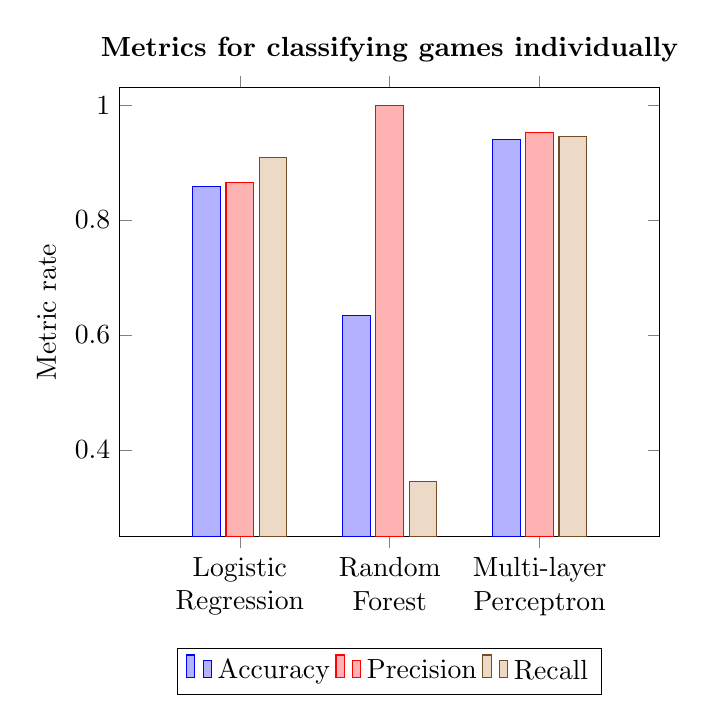
\begin{tikzpicture}
\newaxis{\textbf{Metrics for classifying games individually}}{Metric rate}{0.25}{1.03}

\addplot coordinates {(Logistic Regression,0.8589) (Random Forest,0.6347) (Multi-layer Perceptron,0.93947)};
\addplot coordinates {(Logistic Regression,0.8651) (Random Forest,1.0) (Multi-layer Perceptron,0.95256)};
\addplot coordinates {(Logistic Regression,0.909) (Random Forest,0.34545) (Multi-layer Perceptron,0.94545)};
\legend{Accuracy,Precision,Recall}

\end{axis}
\end{tikzpicture}
\caption{Training results of classifying each game. Note that the size of the dataset is reduced significantly compared to the previous classification approach because there are only a small number of games.}
\end{figure}

% Random forest gets perfect precision but low recall, hence likely predicting a very few positive results (shown by low recall), but always get the positive prediction correct (perfect precision)




\subsection{Game statistic features}

\subsection{Itemisation features}

\subsection{Combining features}


\end{document}
